\documentclass[a4paper,11pt,titlepage]{article}

%Εισαγωγή γλωσσικής υποστήριξης
%ελληνικό hyphenation

\usepackage{fontspec}
\usepackage{xunicode}
\usepackage{xltxtra}
\usepackage{xgreek}
\usepackage[colorlinks]{hyperref}
\usepackage{enumerate}
\usepackage{amsmath}
%η γραμματοσειρά
%\setmainfont[Mapping=tex-text]{Times New Roman} %απλοποιημένο σε σχέση με το άρθρο
\setmainfont[Mapping=tex-text]{Linux Libertine} 
%page orientation
\usepackage{a4wide}
\voffset = -0.5in
\textheight = 664pt

%Custom commands
\newcommand{\supscript}[1]{\ensuremath{^{\textrm{#1}}}}
\newcommand{\subscript}[1]{\ensuremath{_{\textrm{#1}}}}
\newcommand{\degrees}{^{\circ}}
\newcommand{\newln}{\\&\quad\quad{}} % for multiline equations within a split environment

%Άλλα χρήσιμα πακέτα
\usepackage{graphicx} 	%εισαγωγή εικόνων jpg/png κλπ
\usepackage{listings}
\lstset{commentstyle=\textit,
captionpos=b,
breakatwhitespace=true,
showstringspaces=false,
breaklines=true,
keywordstyle=\color{black}\bfseries,
float=htb,
frame=single}

%απενεργοποίηση του indent στις νέες παραγράφους
\parindent=0in

\numberwithin{equation}{section} %αρίθμηση εξισώσεων ανά section

%macro που δίνει το μέγιστο επιτρεπτό μέγεθος σε μια εικόνα χωρίς να παραβιάζει τα όρια του LaTeX
\makeatletter
\def\maxwidth{
\ifdim\Gin@nat@width>\linewidth
\linewidth
\else
\Gin@nat@width
\fi
}
\makeatother


\begin{document}

%\pagestyle{headings}    %αρίθμηση στο πάνω μέρος της σελίδας

%\maketitle
\begin{titlepage}
\begin{center}
\includegraphics[width=50mm]{pyrforos.pdf}\\[0.5cm]
\textbf{\LARGE ΕΘΝΙΚΟ ΜΕΤΣΟΒΙΟ ΠΟΛΥΤΕΧΝΕΙΟ}\\
\textrm{\Large Σχολή Εφαρμοσμένων Μαθηματικών και Φυσικών Επιστημών}\\[2.0cm]
\Huge{Φυσική και Τεχνολογία των laser\\}
\Large{\textit{$6^o$} εξάμηνο, ΣΕΜΦΕ}\\[2.0cm]
\Large{\textit{\textbf{Ασκήσεις}}}\\[5.0cm]
\normalsize

\vfill
%bottom of the page
{Αθήνα, 2012}

\end{center}
\end{titlepage}
\tableofcontents
\newpage

\section{Άσκηση 1}
Υπολογίστε τη συχνότητα($Hz$), τον κυματαριθμό($cm^{-1}$) και την ενέργεια ενός φωτονίου μήκους κύματος $\lambda=1{\mu}m$ στο κενό.

\subsection*{\underline{Λύση:}}

Στο κενό έχουμε 

\begin{equation}
 \lambda\nu=c
\end{equation}
 και επομένως

\begin{equation}
 \nu=\frac{\lambda}{c}=3\times10^{14} Hz
\end{equation}
άρα
\begin{equation}
 E=h\nu=1.99\times10^{-19}J
\end{equation}

Λόγω του ότι $1eV=1.6\times10^{-19}J$ προκύπτει ότι $E=1.24eV$, δηλαδή ίση με την κινητική ενέργεια ενός ηλεκτρονίου που έχει επιταχυνθεί  από μία διαφορά δυναμικού $1.24eV$. Το αντίστροφο μήκος κύματος (κυματαριθμός) είναι $\widetilde{u}=\nu/c$ και χρησιμοποιείται συχνά με την έννοια της συχνότητας και εκφυλίζεται σε $cm^{-1}$, δηλαδή  

\begin{equation}
\widetilde{N}=\frac{\nu}{c}=10^4cm^{-1} 
\end{equation}

\textbf{Σημείωση:} Ο τύπος μετατροπής ενέργειας $eV$ και μήκους κύματος $\lambda$ (${\mu}m$) είναι

\begin{equation}
 E(eV)=\frac{1.24}{\lambda({\mu}m)}
\end{equation}

Ο κυματαριθμός είναι λοιπόν
\begin{equation}
 \widetilde{N}=\nu/c=\frac{E}{hc}
\end{equation}

$1cm^{-1}\sim1.24\times10^{-4}eV$\\ $1eV\sim8065.5 cm^{-1}$

\newpage
\section{Άσκηση 2}

Υπολογίστε σε κυματαριθμούς την ενέργεια ${\Delta}E=kT$, όπου $k$ η σταθερά Boltzmann και $T$ η απόλυτη θερμοκρασία ($300K$).

\subsection*{\underline{Λύση:}}

Η θερμική ενέργεια των 300K δίνεται από τον τύπο
\begin{equation}
 kT=4.14\times10^{-21} J
\end{equation}

Η σχέση κυματαριθμού-ενέργειας είναι
\begin{equation}
 \widetilde{u}=\frac{\nu}{c}=\frac{E}{hc}=\frac{kT}{hc}=208.5 cm^{-1}
\end{equation}

\section{Άσκηση 3 (ασκ.1.3 από λυσάρι)}

Αν τα επίπεδα 1 και 2 ενός κβαντικού συστήματος είναι διαχωρισμένα από ενέργεια $E_2-E_1$ τέτοια που η αντίστοιχη συχνότητα μετάπτωσης εμπίπτει στο μέσο της ορατηής περιοχής, υπολογίστε το λόγο των πληθυσμών των δύο επιπέδων σε θερμική ισορροπία σε θερμοκρασία δωματίου.

\subsection*{\underline{Λύση:}}
Σε περίπτωση θερμικής ισορροπίας, οι πληθυσμοί επιπέδων περιγράφονται από τη στατιστική Boltzmann. Παίρνοντας $\lambda=0.55{\mu}m$, σαν το μέσο της ορατής περιοχής, αντιστοιχεί σε συχνότητα $18.181cm^{-1}$. Η εξίσωση της στατιστικής Boltzmann είναι:

\begin{equation}
\frac{N^e_2}{N^e_1}=exp[-\frac{E_2-E_1}{kT}]=1.1\times10^{-38}
\end{equation}

όπου $kT=208cm^{-1}$, $E_2-E_1=18.181cm^{-1}$

\begin{quote}
 \textbf{Σημείωση:} 
\begin{itemize}
 \item Όταν βλέπουμε άσκηση με θερμική ισορροπία, σκεφτόμαστε αμέσως τη στατιστική Boltzmann
\begin{equation}
exp[-\dfrac{E_2-E_1}{kT}]=\dfrac{N_2}{N_1}
\end{equation}
 \item Στην περιοχή του ορατού παίρνουμε όποιο $\lambda$ μας βολεύει ($0.5-1{\mu}m$).
\end{itemize}
\end{quote}

\newpage
\section{Άσκηση 4 (ασκ.1.4 από λυσάρι)}

Σε κατάσταση θερμικής ισορροπίας ($T=300K$), ο λόγος των πληθυσμών των επιπέδων $N_2/N_1$ για κάποιο ιδιαίτερο ζεύγος επιπέδων δίνεται από το $1/e$. Υπολογίστε τη συχνότητα για αυτή τη μετάπτωση. Σε ποια περιοχή Η.Μ. φάσματος εμπίπτει αυτή η συχνότητα;

\subsection*{\underline{Λύση:}}

Από την εξίσωση της στατιστικής Boltzmann στην περίπτωση που $N_2/N_1=1/e$ έχουμε,

\begin{equation}
 E_2-E_1=kT
\end{equation}
η οποία για θερμοκρασία δωματίου δίνει:

\begin{equation}
 E_1-E_2=208cm^{-1}
\end{equation}

Αυτός ο ενεργειακός διαχωρισμός αντιστοιχεί σε $\lambda=49{\mu}m$ (υπέρυθρο, όχι μεσαίο υπέρυθρο).
\newpage
\section{Άσκηση 5}

Προσδιορίστε το λόγο των πληθυσμών, σε θερμική ισορροπία δύο επιπέδων που απέχουν κατά ενέργεια ${\Delta}E$ ίση με:
\begin{enumerate}
 \item$10^{-4}eV$ τιμή που ισοδυναμεί με την απόσταση δύο περιστροφικών επιπέδων πολλών μορίων 
 \item$5\times10^{-2}eV$ τιμή που ισοδυναμεί με τα μοριακά δονητικά επίπεδα
 \item$3eV$ τιμή που αντιστοιχεί στην τάξη μεγέθους της ηλεκτρονικής διέγερσης ατόμων
\end{enumerate}
Θεωρήστε ότι τα δύο επίπεδα έχουν τον ίδιο εκφυλισμό και ότι η θερμοκρασία είναι 100Κ, 300Κ (δωματίου) και 1000Κ.
\subsection*{\underline{Λύση:}}
Ο λόγος των πληθυσμών δύο επιπέδων σε θερμική ισορροπία που απέχουν κατά \\${\Delta}E=E_2-E_1>0$ δίνεται από την:

\begin{equation}
\dfrac{N_2}{N_1}=\dfrac{g_2}{g_1}exp[-\dfrac{{\Delta}E}{kT}]
\end{equation}

\begin{tabular}{l | l}
\hline
 $N_1,N_2$ & οι πληθυσμοί\\
 $g_1,g_2$ & οι εκφυλισμοί των δύο επιπέδων\\
\hline
\end{tabular}
\\[0.5cm]
Από την παραπάνω εξίσωση και ξέροντας πως $g_1=g_2$ έχουμε:

\begin{table}[h!]
\begin{center}
    \begin{tabular}{ | c | c | c | c | p{5cm} |}
    \hline
     ${\Delta}E (eV)$	& $T=100K$		& $T=300K$ 		& $T=1000K$		& Σχόλια\\ \hline
     $10^{-4}$		& $0.9885$		& $0.9962$		& $0.9988$		& Ίδιοι πληθυσμοί, εύκολη αντιστροφή\\ \hline
     $5\times10^{-2}$	& $9\times10^{-3}$	& $1.45\times10^{-1}$	& $5.6\times10^{-1}$	& Μερικοί πληθυσμοί στο $2^ο$ επίπεδο, αρκετή προσπάθεια για αντιστροφή. Πρέπει να ξεφύγει από θερμική ισορροπία και να πάει σε υψηλές θερμοκρασίες\\ \hline
     $3$ & $5\times10^{-184}$	& $8\times10^{-49}$	& $8\times10^{-16}$	& Πολύ δύσκολη η αντιστροφή πληθυσμών. Αμελητέοι πληθυσμοί στο $2^ο$ επίπεδο.\\ \hline
    \end{tabular}
\end{center}
\end{table}
\newpage
\section{Άσκηση 6 (ασκ.1.6 από λυσάρι)}

Η δέσμη ενός laser ρουβιδίου ($\lambda=0.694{\mu}m$), στέλνεται προς τη σελήνη αφού περάσει από τηλεσκόπιο διαμέτρου $1m$. Υπολογίστε τη διάμετρο $D_m$ της δέσμης στη σελήνη υποθέτοντας πως η δέσμη έχει τέλεια χωρική συμφωνία (η απόσταση μεταξύ γης-σελήνης είναι περίπου $384.000km$).
\subsection*{\underline{Λύση:}}

Το μέγεθος της δέσμης στη σελήνη ορίζεται από την απόσταση δέσμης $\theta_d$. Σύμφωνα με την παρακάτω σχέση και θέτοντας $\beta=1$, βρίσκουμε:
\begin{equation}
 \theta_d=\frac{\beta\lambda}{D}=0.694\times10^{-6} rad
\end{equation}

όπου D είναι η διάμετρος του τηλεσκοπίου. Έτσι η διάμετρος της δέσμης στη σελήνη δίνεται από:
\begin{equation}
 D_m=2Ltan{\theta_d}=2L\theta_d=532m
\end{equation}
όπου L η απόσταση γης-σελήνης.

\textbf{Σημείωση:} Η διάμετρος του τελευταίου οπτικού στοιχείου που περνάει η δέσμη laser λέγεται διάμετρος πηγής.

\section{Άσκηση 7}

Δέσμη laser ισχύος $P_l=10W$ εστιάζει σε φωτεινή κηλίδα διαμέτρου $d=1mm$, πάνω σε μία απόλυτα απορροφητική επιφάνεια-στόχο. Υπολογίστε την πίεση ακτινοβολίας $P_t$ πάνω στο στόχο.

\subsection*{\underline{Λύση:}}

Η ένταση της δέσμης είναι ίση με 
\begin{equation}
I=4P_l/{\pi}d_2=1.27\times10^{13} Wm^{-2}
\end{equation}
όπου ${\pi}d^2/4$ το εμβαδό της εστιασμένης δέσμης. Επομένως η πίεση της ακτινοβολίας πάνω στο στόχο είναι:
\begin{equation}
 P_t=\frac{I}{c}=4.2\times10^4Pa=0.42 bar
\end{equation}
η οποία είναι συγκρίσιμη με την ατμοσφαιρική.
\newpage
\section{Χρόνος και μήκος συμφωνίας ασύμφωνης μονοχρωματικής ακτινοβολίας}
Χρησιμοποιούμε ένα φίλτρο συμβολής με ζώνη διέλευσης $10nm$ στα $500nm$ για να πετύχουμε μονοχρωματικό φως από πηγή λευκού φωτός. Υπολογίστε το χρόνο και το μήκος συμφωνίας του μονοχρωματικού φωτός.

\subsection*{\underline{Λύση:}}

Αν ο χρόνος συμφωνίας ΗΜ κύματος είναι $\tau_0$ τότε το εύρος ζώνης αντίστοιχα είναι $\Delta\nu_0\simeq 1/\tau_0$. Επομένως αντίστροφα αν το εύρος ζώνης είναι $\Delta\nu_0$ ο αντίστοιχος χρόνος συμφωνίας είναι $\tau_0=1/\Delta\nu_0$. Χρησιμοποιώντας τη σχέση $c=\lambda\nu$ έχουμε:
\begin{equation}
 |\Delta\nu|=\frac{c}{\lambda^2}|\Delta\lambda|
\end{equation}

\begin{equation}
 \tau_0=\frac{1}{\Delta\nu}=\frac{\lambda^2}{c\Delta\lambda}=83fs
\end{equation}

Το μήκος συμφωνίας είναι:
\begin{equation}
 \lambda_c=c\tau_0=\frac{\lambda^2}{\Delta\lambda}=2.5\times10^{-5}m
\end{equation}


\section{Άσκηση 9}

Laser με οπτικό αντηχείο αποτελείται από δύο κάτοπτρα με ακτίνα καμπυλότητας $R=R_1=R_2=200mm$. Λόγω κατασκευαστικών σφαλμάτων οι πραγματικές ακτίνες καμπυλότητας είναι $R_1=R+{\Delta}R$  και $R_2=R-{\Delta}R$, όπου ${\Delta}R=3mm$. Τα laser λειτουργεί σωστά όταν τα κάτοπτρα τοποθετηθούν σε μικρότερη ή μεγαλύτερη απόσταση από την ομοεστιακή θέση. Εξηγήστε αυτή την πειραματική διαπίστωση και προσδιορίστε ακριβώς την απόσταση για την οποία το laser αρχίζει να λειτουργεί.

\subsection*{\underline{Λύση:}}
Για $L=R=200mm$ οι παράμετροι σταθερότητας του αντηχείου είναι:


\begin{equation}
 g_1=1-\frac{R}{R+{\Delta}R}>0
\end{equation} 

 \begin{equation}
 g_2=1-\frac{R}{R-{\Delta}R}<0
\end{equation} 

άρα για $g_1g_2<0$, το οπτικό αντηχείο είναι ασταθές. Θα πρέπει λοιπόν:

\begin{equation}
 g_1g_2>0\Rightarrow(1-\frac{R}{R+{\Delta}R})(1-\frac{R}{R-{\Delta}R})>0\Rightarrow L^2-2RL+({R+{\Delta}R})({R-{\Delta}R})>0
\end{equation}

Η παραπάνω ανίσωση ικανοποιείται για 

\begin{enumerate}
 \item $L>R+\Delta R$
 \item $L<R-\Delta R$ 
\end{enumerate}


Επομένως θα πρέπει τα κάτοπτρα να μετακινηθούν κατά $3mm$ προς τα μέσα ή προς τα έξω από την ομοεστιακή σχέση.

\section{Άσκηση 10}

Δείξτε ότι η πίεση ακτινοβολίας μίας φωτεινής δέσμης έντασης $I$ που προσπίπτει κάθετα σε μία απόλυτα απορροφητική επιφάνεια είναι $I/c$. Η ορμή φωτονίου συχνότητας $V$ δίνεται $q=(h/2\pi)/k$ και $k=2\pi\nu/c$.

\subsection*{\underline{Λύση:}}

Η συνολική ορμή διατηρείται και κάθε φωτόνιο μεταφέρει την ορμή του στην επιφάνεια. Αν $\Phi$ η ροή των φωτονίων, τότε η συνολική ορμή σε επιφάνεια ${\Delta}s$ σε χρόνο $\Delta t$ είναι:

\begin{equation}
 Q=\Phi q\Delta s\Delta t
\end{equation}

Η δύναμη που ασκείται στη $\Delta s$ είναι $Q=F\Delta t$ και η πίεση:

\begin{equation}
 P=\dfrac{F}{\Delta s}=\dfrac{Q}{\Delta s\Delta t}=\Phi q=\dfrac{\Phi h\nu}{c}
\end{equation}

Άρα, αφού $I=\Phi h\nu$, έχουμε ότι $P=I/c$.

\textbf{Σημείωση:}
\begin{itemize}
 \item Αν η επιφάνεια είναι ανακλαστική τότε $P=2I/c$ και το φωτόνιο κατά την ανάκλαση έχει φορτίο $\Delta q=q-(-q)=2q$.
 \item Αν έχουμε πρόσπτωση υπό γωνία $\theta$ τότε η ορμή είναι ίση με 
\begin{equation}
Q=\Phi q\Delta \cos\theta \Delta t 
\end{equation}
και άρα η πίεση ισούται με
\begin{equation}
 P=\dfrac{\Phi \cos\theta}{\Delta t}=\Phi q\cos^2\theta=\dfrac{I}{c\cos^2\theta}
\end{equation}
\end{itemize}


\section{Άσκηση 11} 

Έχουμε ενεργό υλικό μήκους $5cm$  με συντελεστή ενίσχυσης $g_0=5m^{-1}$ και ένταση κορεσμού $5Wm^{-2}$. Μονοχρωματική ΗΜ ακτινοβολία περνάει μέσα  από το ενεργό υλικό με ένταση $10Wm^{-2}$. Υπολογίστε την ένταση εξόδου.

\subsection*{\underline{Λύση:}}

Η αύξηση της ροής $F$ των φωτονίων μετά από καθυστέρηση $dz$ είναι $dF=gFdz$. Επειδή $F=I/h\nu$ ισχύει ότι:
\begin{equation}
 dI=gIdz
\end{equation}

όπου $g$ ο συντελεστής ενίσχυσης και υπολογίζεται από την:
\begin{equation}
 g=\frac{g_0}{1+\dfrac{I}{I_s}}
\end{equation}

όπου $I_s$ η ένταση κορεσμού.
\\
Από τις παραπάνω 2 εξισώσεις έχουμε:

\begin{equation}
(\dfrac{1}{I}+\dfrac{1}{I_s})dI=g_0dz
\end{equation}

Για $I=I_0$ $(z=0)$, έχουμε:
\begin{equation}
 I=I_0\exp ( g_0\ell-\dfrac{I-I_0}{I_s} )
\end{equation}

όπου $\ell$ το μήκος του ενεργού υλικού. \\
Αν ο κορεσμός είναι αμελητέος, στην έξοδο θα έχουμε:

\begin{equation}
 I=I_0\exp(g_0\ell)=12.84Wm^{-2}
\end{equation}


\section{Άσκηση 12 (ασκ.9.23 από λυσάρι)}

Να διερευνηθούν οι δυνατότητες μέγιστης αντίστασης και ακρίβειας μέτρησης ενός μετρητή αποστάσεων laser διαφοράς φάσης, με κρύσταλλο χαλαζία μέγιστης συχνότητας $f_{max}=4.433MHz$ και ελάχιστης συχνότητας $f_{min}=80Hz$.

\subsection*{\underline{Λύση:}}

Σε μία τέτοια διάταξη, ο χρόνος που μεσολαβεί από την εκπομπή μέχρι τη λήψη της ακτινοβολίας laser ισούται με $t=2r/c$, όπου r η μετρούμενη απόσταση. Η αντίστοιχη μετατόπιση φάσης είναι $\phi=2\pi ft$, όπου $f$ η συχνότητα του κρυστάλλου. Επομένως

\begin{equation}
 \phi= \frac{4\pi rf}{c}
\end{equation}

\begin{itemize}
 \item Για $4.433MHz$ και (πχ) $r=10m$
\end{itemize}

\begin{equation}
 \phi=\frac{4\pi \times10m \times 4.433\times10^{-6}s^{-1}}{3\times10^8ms^{-1}}=0.5911\times\pi=106\degrees
\end{equation}

Λόγω του τύπου του κυκλώματος που έχουμε σε αυτές τις διατάξεις, η μέγιστη τιμή της $\phi$ είναι $\phi=\pi=180\degrees$. Επομένως η μέγιστη απόσταση που μπορεί να μετρήσει κανείς στα $4.433MHz$ είναι:

\begin{equation}
 r_{max}=\frac{\phi c}{4\pi f}=\frac{\pi\times 3\times10^8ms^{-1}}{4\pi\times 4.433\times10^{6} s^{-1}}=16.9m
\end{equation}

\begin{itemize}
 \item Για $80Hz$ και (πχ) $r=10m$
\end{itemize}

$\phi=\pi=180\degrees$ και 

\begin{equation}
 r^{'}_{max}=\frac{\phi c}{4\pi f}=\frac{\pi\times 3\times10^8ms^{-1}}{4\pi\times 80s^{-1}}=937.5 km
\end{equation}

\begin{itemize}
 \item Ακρίβεια
\end{itemize}

Αν η ελάχιστη ανιχνεύσιμη διαφορά φάσης είναι $\Delta\phi=\pm1/4\degrees$ και η μέγιστη συχνότητα $f_{max}=4.433MHz$ τότε η ελάχιστη ανιχνεύσιμη απόσταση είναι η 

\begin{equation}
 \Delta r=\frac{\Delta tc}{2}=\frac{\Delta\phi c}{4\pi f}=\frac{\pm 0.25\degrees\times 3\times10^8ms^{-1}}{4\times 180\degrees \times 4.433\times10^6s^{-1}}=\pm\frac{75}{3192}=2.3cm
\end{equation}

Αν η ελάχιστη ανιχνεύσιμη διαφορά φάσης είναι $\Delta\phi=\pm1/4\degrees$ και η ελάχιστη συχνότητα $f_{min}=80Hz$ τότε η ελάχιστη ανιχνεύσιμη απόσταση είναι η 

\begin{equation}
 \Delta r=\frac{\Delta tc}{2}=\frac{\Delta\phi c}{4\pi f}=\frac{\pm 0.25\degrees\times 3\times10^8ms^{-1}}{4\times 180\degrees \times 80s^{-1}}=\pm\frac{0.75\times10^8m}{57600}=1.3km
\end{equation}

\section{Άσκηση 13 (ασκ.9.24 από λυσάρι)}

Ο πομπός laser τηλεμέτρου ηχούς παλμών εκπέμπει ενέργεια $W_T$. Να βρεθεί η επιστρέφουσα στον ανιχνευτή του τηλεμέτρου ενέργεια $W_r$ μετά από ανάκλαση σε στόχο που βρίσκεται σε απόσταση $R$.

\subsection*{\underline{Λύση:}}

Η εκπεμπόμενη ενέργεια είναι ίση με $W_T$.  Η ενέργεια που φτάνει στο στόχο σε απόσταση $R$ είναι:

\begin{equation}
 W_{tr}=W_T\exp(-\mu R)
\end{equation}

όπου $\mu$ ο συντελεστής ατμοσφαιρικής εξασθένησης. Αν θεωρήσουμε ένα επίπεδο ανακλαστικό στόχο κατά Lambert (ημισφαιρικός) που η κάθετος σ'αυτόν σχηματίζει γωνία $\phi$ με την προσπίπτουσα ακτινοβολία, τότε η ακτινοβολία που ανακλάται μέσα σε κώνο στερεάς γωνίας $\Omega$, σε γωνία $\phi$ ως προς την κάθετο είναι:

\begin{equation}
 W_{te}=\frac{W_{tr}(p \cos\phi)\Omega }{\pi}
\end{equation}

όπου $p$ η ανακλαστικότητα του στόχου. \\[0.3cm]
Το σύστημα λήψης του τηλεμέτρου διαμέτρου $D$ που βρίσκεται σε απόσταση $R$ από το στόχο, βλέπει σε μία στερεά γωνία $\Omega=\pi D^2/4R^2$. Επειδή $\omega\geq \alpha$, όπου $\omega$ το πεδίο παρατήρησης του ανιχνευτή και $\alpha$ το άνοιγμα της δέσμης του laser, η ενέργεια που φτάνει στον ανιχνευτή θα είναι:

\begin{equation}
 W_r=W_{te}\tau\exp(-\mu R)
\end{equation}

όπου $\tau$ η διαπερατότητα των οπτικών της λήψης. Έτσι τελικά:

\begin{equation}
 W_r=\dfrac{W_T p \tau\cos\phi e^{-2\mu R}D^2}{4R^2}
\end{equation}

Αν χρησιμοποιήσει κανείς κάποια χαρακτηριστικά στοιχεία για ένα τηλέμετρο $Nd:YAG$ πχ.
\begin{itemize}
 \item $W_T=10^{-3}J$
 \item $p=1/2$
 \item $\tau=1/2$
 \item $R=20\times10^3m$
 \item $D=0.05m$
 \item $\phi=20\degrees\Longrightarrow \cos\phi=0.94$
 \item $\mu=0.1\times10^{-3}$
\end{itemize}

τότε

\begin{equation}
 W_r=\dfrac{W_T p \tau\cos{\phi}\exp{-2\mu R}D^2}{4R^2}=6.6\times10^{-18}Joule
\end{equation}
ή
\begin{equation}
 P_r=\dfrac{6.6\times10^{-18}J}{10\times10^{-9}s}=0.66nWatt
\end{equation}

\section{Άσκηση 14 (ασκ.9.25 από λυσάρι)}

Προσδιορίστε την απαιτούμενη ισχύ εξόδου ενός τηλεμέτρου laser $Nd:YAG$ ώστε να μπορεί να μετρήσει $5km$ υπό οποιεσδήποτε συνθήκες.

\subsection*{\underline{Λύση:}}

Θεωρούμε ότι ο ανιχνευτής του laser αποτελείται από μία φωτοοδίοδο τύπου, avalanche ή PIN, [C30817], που έχι πολωθεί κατά τέτοιο τρόπο ώστε να έχει σταθερή ευαισθησία και ενισχυτή. Στη χειρότερη περίπτωση ο ανιχνευτής διακρίνει σήματα που προκαλούν ηλεκτρικούς παλμούς 20nA. Για το εύρος των φωτεινών παλμών που παράγει ένα Q-switched laser NdYAG περιμένει κανείς μία απώλεια στον ενισχυτή του σήματος ανίχνευσης κατά ένα παράγοντα 0.65. Επίσης πρέπει να υπάρχει μία σχέση σήματος προς θόρυβο περίπου 8 προς 1, που αντιστοιχεί σε πιθανότητα $99\%$ ανίχνευσης ή ένα λανθασμένο σήμα στα 1000 πραγματικά. Έτσι το ελάχιστο ανιχνεύσιμο σήμα από τον ανιχνευτή του συστήματος ανίχνευσης θα είναι: $20nA\times8/0.65\simeq250nA$. Η ευαισθησία της διόδου θα ρυθμιστεί περίπου σε $10nA/Watt$ κάτι που δίνει μία ελάχιστη ανιχνεύσιμη ισχύ στη δίοδο περίπου $25nWatt$.\\
Αν θεωρήσουμε απόδοαη οπτικού συστήματος $0.5$ και διαπερατότητα φίλτρων $0.8$ τότε η ελάχιστη ανιχνεύσιμη ισχύς κατά την επιστροφή στο τηλέμετρο είναι $25nW/0.5\times0.8=62.5nW$. Αν θεωρήσουμε επίσης τη διάμετρο εισόδου του ανιχνευτή π.χ. $60mm$ τότε πρέπει να φτάνει στο τηλέμετρο μία ένταση ακτινοβολίας $2.3\times10^{-5}W/m^2$. Υποθέτουμε ότι ο στόχος έχει μία κλίση $45\degrees$ ως προς την ακτίνα laser του τηλεμέτρου, μία ανακλαστικότητα $p$ και βρίσκεται σε απόσταση $R$ από το τηλέμετρο. Στην περίπτωση αυτή η επιστρέφουσα ένταση ακτινοβολίας είναι:

\begin{equation}
  W_r=\dfrac{W_T p (\cos\phi)e^{-2\mu R}}{\pi R^2}
\end{equation}

όπου $\mu$ ο συντελεστής ατμοσφαιρικής εξασθένησης. Στη χειρότερη των περιπτώσεων όπου η ανακλαστικότητα του στόχου είναι $0.1$, ο στόχος μας βρίσκεται στα 5km και η ορατότητα είναι περίπου $5\times4km/3$ έχουμε ένα συντελεστή ατμοσφαιρικής εξασθένησης (για την ορατότητα αυτή), $0.28/km$. Για να μπορεί να μετρηθεί ένας τέτοιος στόχος κάτω από αυτές τις συνθήκες πρέπει ο πομπός laser να παράγει ισχύ:

\begin{equation}
 P=\frac{\pi\times(5000)^2}{0.1\times0.7\times0.061}\times2.3\times10^{-5}Watt\simeq0.45Watt
\end{equation}

Για να είναι ασφαλής θα πρέπει κανείς να έχει περιθώριο ενός παράγοντα $\times2$ για ενδεχόμενη μειωμένη, (με την πάροδο του χρόνου), απόδοση του συστήματος, δηλαδή θα πρέπει να παράγει ο πομπός laser τουλάχιστον $0.9MWatt$. Τελικά με έξοδο περίπου $1MWatt$ από το laser, το τηλέμετρο μπορεί να μετρήσει οποιοδήποτε στόχο κάτω από οποιεσδήποτε συνθήκες ορατότητας αν αυτός βρίσκεται μέχρι $5km$ από το τηλέμετρο.

\section{Άσκηση 15 (ασκ.9.12 από λυσάρι)}

Ποια η διαφορά συχνότητας μεταξύ του $TEM_{00}$ και του $TEM_{01}$ για την ίδια τιμή του $q$, αν το μήκος του αντηχείου laser $CO_2$ βιομηχανικών εφαρμογών είναι $L=4m$ και τα $R_1=R_2=20m$;
\begin{enumerate}
 \item Τι ποσοστό της συχνότητας εκπομπής του laser $CO_2$ παριστάνει η διαφορά αυτή;
 \item Τι σημαίνουν οι δείκτες $00$ και $01$ στα $TEM_{00}$ και $TEM_{01}$;
\end{enumerate}

\subsection*{\underline{Λύση:}}

1) Ισχύει ότι:

\begin{equation}
 \nu_{00q}=[q+\frac{\cos^{-1}g}{\pi}]\frac{c}{2L}
\end{equation}
 και 

\begin{equation}
 \nu_{01q}=[q+\frac{2\cos^{-1}g}{\pi}]\frac{c}{2L}
\end{equation}

όπου για την περίπτωσή μας $g_1=g_2=g=1-\dfrac{L}{R}=1-\dfrac{4m}{20m}=0.8$.\\
Άρα

\begin{equation}
\begin{split}
& \Delta \nu=\frac{\cos^{-1}g}{\pi}\times\frac{c}{2L}=\frac{\cos^{-1}0.8}{\pi}\times\frac{3\times10^8msec^{-1}}{8m}= \\
& =\frac{\cos^{-1}0.8\times300}{3.14\times8}MHz=\frac{36.9\times300}{25.12}MHz=440.3MHz
\end{split}
\end{equation}

Τώρα το 
\begin{equation}
 \dfrac{\Delta \nu}{\nu_{00q}}=\dfrac{\cos^{-1}g/\pi}{q+\cos^{-1}/\pi}=\dfrac{\cos^{-1}g}{\pi q+\cos^{-1}g}
\end{equation}

Δεν ξέρουμε το $q$, ξέρουμε όμως ότι το laser $CO_2$ εκπέμπει στα $10.6\mu m$ περίπου, άρα το $\nu_0$ είναι:

\begin{equation}
 \nu_0=\frac{3\times10^8}{10.6\times10^{-6}}sec^{-1}=\frac{300}{10.6}\times10^{14}sec^{-1}=28.3\times10^{14}Hz
\end{equation}

οπότε έχουμε:

\begin{equation}
  \dfrac{\Delta\nu}{\nu_{00q}}=\frac{440.3\times10^6 Hz}{28.3\times10^{14}Hz}=15.6\times10^{-18}\simeq1.6\times10^{-7}
\end{equation}

Μπορούμε επίσης να εκτιμήσουμε και το $q$ αν θέλουμε. Θεωρούμε $q\gg1$ οπότε 

\begin{equation}
\nu\simeq \dfrac{qc}{2L}\longrightarrow q\simeq \dfrac{2L}{\lambda}\longrightarrow q=\dfrac{8m}{10.6\times10^{-6}m}=0.75\times10^6
\end{equation}

πράγματι πολύ μεγάλο.
\\[0.5cm]
2)
\\[0.3cm]
Οι δείκτες $00$ και $01$ αντιπροσωπεύουν μηδενικές εντάσεις κατά μήκος των αξόνων $x$ και $y$ αντίστοιχα.

\newpage
\section{Άσκηση 16}

Θεωρούμε μία οπτική κοιλότητα με 2 κοίλα σφαιρικά κάτοπτρα με ακτίνα καμπυλότητας $R=4m$ σε απόσταση $1m$ το ένα από το άλλο. Υπολογίστε το μέγεθος του ρυθμού $TEM_{00}$ στο κέντρο της κοιλότητας και πάνω στα κάτοπτρα όταν το σύστημα λειτουργεί στα $0.514\mu m$.

\subsection*{\underline{Λύση:}}

\begin{figure}[!h]
\centering
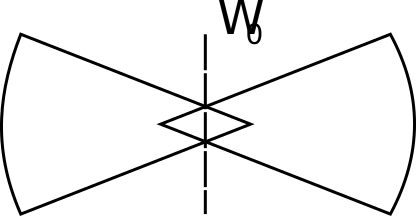
\includegraphics[width=7cm]{katoptra.pdf}\\[0.3cm]
\caption{Κοίλα σφαιρικά κάτοπτρα}
\end{figure}

Έχουμε $g_1=g_2=g=1-\dfrac{L}{R}=0.75$ και $g_1g_2=0.562$ (σταθερή κοιλότητα).

Μέγεθος κηλίδας:
\begin{equation}
 W_0^2=\frac{L\lambda}{\pi}\sqrt{\dfrac{1+g}{4(1-g)}}
\end{equation}

\begin{equation}
 W^2=W_1^2=W_2^2=\frac{L\lambda}{\pi}\sqrt{\dfrac{1}{1-\gamma^2}}
\end{equation}

Οι παραπάνω εξισώσεις ισχύουν για συμμετρική κοιλότητα (μέσο δέσμης $\rightarrow$ μέσο κοιλότητας, αφού $R=R_1=R_2$). \\
Όταν όμως [$R_1=\infty$ ή $g_1=1$] και [$g_1=g_2=1-\frac{L}{R}$]
\\[0.5cm]

\begin{equation} 
 W_0^2=W_1^2=\frac{L\lambda}{\pi}\sqrt{\frac{g}{1-g}}=532
\end{equation} 

\begin{equation} 
 W_2^2=\frac{2\lambda}{\pi}\sqrt{\frac{1}{g(1-g)}}=0.614
\end{equation} 

\newpage
\section{Άσκηση 17}

Δείξτε ότι η ταλαντωτική συχνότητα ενός διατομικού μορίου που αποτελείται από δύο άτομα με μάζες $m_1$ και $m_2$, είναι 
\begin{equation}
\nu=\frac{1}{2\pi}\sqrt{\frac{k_0}{m_r}}
\end{equation}
όπου $k_0$ η σταθερά των ελαστικών δυνάμεων, και $m_r$ η ανηγμένη μάζα με $\frac{1}{m_r}=\frac{1}{m_1}+\frac{1}{m_2}$.

\subsection*{\underline{Λύση:}}

Θεωρούμε ότι τα δύο άτομα συνδέονται μεταξύ τους με ελατήρια ελαστικής σταθεράς $k_0$. Η κάθε μία εξίσωση κίνησης, στον άξονα $x$ είναι:

\begin{equation}
 m_1\dfrac{d^2x_1}{dt^2}=k_0(x_2-x_1)
\end{equation}

\begin{equation}
 m_2\dfrac{d^2x_2}{dt^2}=-k_0(x_2-x_1)
\end{equation}

Διαιρώντας την 17.2 με $m_1$, την 17.3 με $m_2$ και διαιρώντας κατα μέλη έχουμε:

\begin{equation}
 \dfrac{d^2(x_2-x_1)}{dt^2}=-k_0(\dfrac{1}{m_1}+\dfrac{1}{m_2})(x_2-x_1)
\end{equation}

Θέτοντας $y=x_2-x_1$ και $\frac{1}{m_r}=\frac{1}{m_1}+\frac{1}{m_2}$, έχουμε:

\begin{equation}
 \dfrac{d^2y}{dt^2}+\dfrac{k_0}{m_r}y=0
\end{equation}

Λύνοντας την παραπάνω διαφορική εξίσωση οδηγούμαστε στα εξής:

%%
%%
\begin{tabular}{ l | l }
\hline
&\\
$ \nu=\dfrac{1}{2\pi}\sqrt{-\dfrac{k_0}{m_r}}$ & Εξίσωση αρμονικού ταλαντωτή με μάζα $m_r$ και ελαστική σταθερά $k_0$.\\  
&\\ 
\hline
&\\
$ \nu=\dfrac{1}{2\pi}\sqrt{\dfrac{2k_0}{M}}$   & Ειδική περίπτωση του διατομικού μορίου $M=m_1=m_2$.\\ 
&\\
\hline
\end{tabular}

\newpage
\section{Άσκηση 18}

Έχει παρατηρηθεί ότι η ταλαντωτική συχνότητα του laser $I_2$ είναι $\widetilde{\nu}=2/3cm^{-1}$. Γνωρίζοντας ότι η μάζα του ατόμου του ιωδίου είναι $m=21.08\times10^{-26}kg$, βρείτε βρείτε την ελαστική σταθερά του ατόμου του ιωδίου.

\subsection*{\underline{Λύση:}}

Η ταλαντωτική συχνότητα του $I_2$ των $2/3cm^{-1}$ αντιστοιχεί από την 
\begin{equation}
 \widetilde{\nu}=\frac{\nu}{c}=\frac{1}{\lambda}
\end{equation}

 άρα

\begin{equation}
 \nu=\widetilde{\nu}c=\frac{2}{3}cm^{-1}\times3\times10^{10}cm s^{-1}=6.4\times10^{12}Hz
\end{equation}

Χρησιμοποιώντας την εξίσωση του προγούμενου προβλήματος, έχουμε:

\begin{equation}
 \nu=\dfrac{1}{s\pi}\sqrt{\dfrac{2k_0}{M}}\Rightarrow k_0=4\pi^2\nu^2\dfrac{m}{2}=170N/m
\end{equation}

\section{Άσκηση 19}

Ένα laser $Nd:YAG$ ($\lambda=1064nm$) με διάμετρο $d=6mm$ και σταθερό προφίλ έντασης, έχει άνοιγμα δέσμης $\theta\simeq3mrad$. Δείξτε ότι η δέσμη του laser δεν είναι περιθλαστικά περιορισμένη.

\subsection*{\underline{Λύση:}}

Το άνοιγμα δέσμης μίας περιθλαστικά περιορισμένης δέσμης δίνεται από την εξίσωση:

\begin{equation}
 \theta^{'}_d=1.22\dfrac{\lambda}{d}=0.216mrad
\end{equation}

Εφ' όσον το $\theta>\theta^{'}$ η δέσμη δεν είναι περιθλαστικά περιορισμένη.
\newpage
\section{Άσκηση 20}

Στην επιφάνεια της γης, η ένταση του ήλιου είναι περίπου $1kWm^2$. Υπολογίστε την ένταση στον αμφιβληστροειδή μας όταν παρατηρούμε απ' ευθείας τον ήλιο χωρίς προστατευτικά γυαλιά. Θεωρήστε ότι:
\begin{enumerate}
 \item η κόρη του ματιού τη μέρα έχει διάμετρο $d=2mm$
 \item η εστιακή απόσταση του ματιού μας είναι $22.5mm$
 \item ο ήλιος παρατηρείται σε γωνία $0.5\degrees$
\end{enumerate}

Συγκρίνετε αυτή την ένταση με αυτή που προκύπτει όταν παρατηρήσουμε απ' ευθείας ένα laser $He-Ne$ διαμέτρου $2mm$.

\subsection*{\underline{Λύση:}}

Αρχικά έχουμε ότι το μήκος κύματος του $He-Ne$ είναι $\lambda=632.8nm$ και η διάμετρος μίας εστιασμένης δέσμης με φακό εστιακής απόστασης $f$ μπορεί να υπολογιστεί από τη σχέση:

\begin{equation}
 D_f=\dfrac{4f\lambda}{\pi D_0}
\end{equation}

όπου $D_O$ η διάμετρος δέσμης πάνω στο φακό εστίασης. Το εμβαδό της κόρης του ματιού είναι:

\begin{equation}
 A=\dfrac{\pi D^2}{4}=3.14mm^2
\end{equation}

Η ισχύς του ήλιου που περνά μέσα από την κόρη του ματιού είναι $P=3.14mW$. Επειδή η εστιακή απόσταση του ματιού μας είναι $f_E=22.5mm$ και επειδή ο ήλιος παρατηρείται υπό γωνία $0.5\degrees$, το είδωλο του ήλιου στον αμφιβληστροειδή έχει διάμετρο:

\begin{equation}
 D_s=2f_E\tan(\theta_s/2)=0.2mm
\end{equation}


Η ένταση ακτινοβολίας στον αμφιβληστροειδή είναι τότε:

\begin{equation}
 I_s=\dfrac{4P}{4D_s^2}=10^5Wm^/m^2
\end{equation}

Στην περίπτωση του $1mW$ $He-Ne$ με $\lambda=638.2nm$, η διάμετρος του ειδώλου στον αμφιβληστροειδή είναι

\begin{equation}
 D_L=\dfrac{4f_E\lambda}{\pi D_O}=9\mu m
\end{equation}

Επομένως η ένταση ακτινοβολίας στον αμφιβληστροειδή είναι 

\begin{equation}
 I_L=\dfrac{4P_L}{\pi D_L^2}=1.6\times10^7W/m^2
\end{equation}

Δηλαδή, ένταση 160 φορές μεγαλύτερη από την περίπτωση του ήλιου. Την επόμενη φορά λοιπόν που θα στρέψετε δέσμη laser στο πρόσωπο του άλλου, σκεφτείτε το περισσότερο...

\newpage

\section{Ρυμοί αυθόρμητης και εξαναγκασμένης εκπομπής}
Για ένα σύστημα σε θερμική ισορροπία υπολογίστε τη θερμοκρασία στην οποία εξισώνονται οι ρυθμοί αυθόρμητης και εξαναγκασμένης εκπομπής για το μήκος κύματος $500nm$. Επίσης να βρεθεί το μήκος κύματος στο οποίο οι ρυθμοί εξισώνονται σε $T=4000K$.

\subsection*{\underline{Λύση:}}

Ο λόγος του ρυθμού αυθόρμητης εκπομπής Α προς το ρυθμό εξαναγκασμένης εκπομπής W, δίνεται από:
\begin{equation}
 R=\dfrac{A}{W}=\dfrac{A}{B\rho{_\nu{_0}}}
\end{equation}
όπου $\rho{_\nu{_0}}$ η πυκνότητα της ενέργειας. Ο A/B δίνεται από την εξίσωση του Einstein:
\begin{equation}
 \frac{A}{B}=\frac{8{\pi}hN_0^3n^3}{c^3}
\end{equation}

H πυκνότητα της ενέργειας δίνεται από τη εξίσωση του Planck:
\begin{equation}
 \rho_\nu=\frac{8\pi\nu^2}{c^3}\frac{h\nu}{exp(h\nu/kT)-1}
\end{equation}
Έτσι έχουμε:
\begin{equation}
 R=exp[\frac{N_0}{kT}-1]=exp[\frac{hc}{kT\lambda}]-1
\end{equation}

Επομένως η θερμοκρασία για την οποία έχουμε $R=1$ είναι και μήκος κύματος $\lambda=500nm$:
\begin{equation}
 T=\dfrac{hc}{k{\lambda}ln2}=41562K
\end{equation}

Το μήκος κύματος στο οποίο οι ρυθμοί εξισώνονται σε $T=4000K$, είναι:
\begin{equation}
 \lambda=\frac{hc}{kTln2}=5.2{\mu}m
\end{equation}
\newpage
\section{Συνθήκη σταθερότητας για οπτική κοιλότητα με κοίλα κάτοπτρα}

Θεωρήστε μία οπτική κοιλότητα που αποτελείται από δύο κοίλα κάτοπτρα τα οποία βρίσκονται μεταξύ τους σε απόσταση $L$\footnote{Συνήθως αναφέρεται και ως οπτικό αντηχείο απόστασης  L.}.
\begin{enumerate}[(i)]
 \item Βρείτε τις τιμές του $L$ για τις οποίες η κοιλότητα είναι σταθερή.
 \item Ποια η περιοχή σταθερότητας για το ίδιο αντηχείο αλλά με κυρτά κάτοπτρα.
\end{enumerate}

\subsection*{\underline{Λύση:}}

Ισχύει ότι:

\begin{itemize}
 \item $R_1>0$
 \item $R_2>0$
 \item $R_1<R_2$
\end{itemize}

και επίσης ξέρουμε ότι:

\begin{equation}
 0<g_1g_2<1
\end{equation}

\begin{equation}
  g_1=1-\dfrac{L}{R_1}
\end{equation}

\begin{equation}
  g_2=1-\dfrac{L}{R_2}
\end{equation}

Σπάμε την ανισότητα 22.1 στα δύο.\\[0.5cm]

\textbf{\underline{1η ανισότητα:}}
\begin{equation}
 (1-\dfrac{L}{R_1})(1-\dfrac{L}{R_2})>0\Longrightarrow\dfrac{L^2}{R_1R_2}-L(\dfrac{1}{R_1}+\dfrac{1}{R_2})+1>0
\end{equation}
\\[0.3cm]
η οποία μας δίνει $L<R_1 $ και $L>R_2$.\\[0.5cm]

\textbf{\underline{2η ανισότητα:}}
\begin{equation}
 (1-\dfrac{L}{R_1})(1-\dfrac{L}{R_2})<1\Longrightarrow\dfrac{L^2}{R_1R_2}-L(\dfrac{1}{R_1}+\dfrac{1}{R_2})<1
\end{equation}

η οποία μας δίνει $L>0$ και $L<R_1+R_2$.

Έτσι οδηγούμαστε στο συμπέρασμα πως υπάρχουν 2 περιοχές σταθερότητας:
\begin{enumerate}[(i)]
 \item $0<L<R_1$
 \item $R_2<L<R_1+R_2$
\end{enumerate}

Στην περίπτωση όπου τα κάτοπτρα είναι κυρτά, ισχύει ότι $R_1<0$, $R_2<0$ και $g_1>L$, $g_2>L$. Άρα $g_1g_2>1$ οπότε το οπτικό αντηχείο είναι ασταθές.
\newpage
\section{Οπτικό αντηχείο με κοίλο και κυρτό κάτοπτρο (1)}

Θεωρήστε ένα οπτικό αντηχείο με ένα κυρτό κάτοπτρο $R_1$ και ένα κοίλο κάτοπτρο $R_2$, που βρίσκονται σε απόσταση $L$. Βρείτε τις τιμές του $L$ για τς οποίες η οπτική κοιλότητα είναι σταθερή. Θεωρήστε δύο περιπτώσεις:
\begin{enumerate}[(i)]
 \item $|R_1|>R_2$
 \item $|R_1|<R_2$
\end{enumerate}

\subsection*{\underline{Λύση:}}

Για να είναι σταθερή η οπτική κοιλότητα θα πρέπει να ισχύουν τα παρακάτω:

\begin{equation}
 0<g_1g_2<1
\end{equation}

\begin{equation}
  g_1=1-\dfrac{L}{R_1}
\end{equation}

\begin{equation}
  g_2=1-\dfrac{L}{R_2}
\end{equation}
\\[0.5cm]

Έχουμε $R_1<0$ άρα $g_1>0$ για όλες τις τιμές του $L$, οπότε $g_1g_2>0\rightarrow g_2>0\rightarrow L<R_2$. Αντικαθιστώντας τα $g_1$ και $g_2$ στην εξίσωση 23.1 έχουμε:

\begin{equation}
\begin{split}
  (1-\dfrac{L}{R_1})(1-\dfrac{L}{R_2})&<1\Rightarrow\\
\Rightarrow \dfrac{L}{R_1R_2}&<\dfrac{1}{R_1}\dfrac{1}{R_2}\Rightarrow\\
\Rightarrow \dfrac{L}{R_1R_2}&<\dfrac{R_1+R_2}{R_1R_2}
\end{split}
\end{equation}

Σε αυτό το σημείο προσοχή. Πολλαπλασιάζουμε κάθε μέλος με το $R_1R_2$, αλλά επειδή το $R_1<0$ (κυρτό) και $R_2>0$ (κοίλο), τότε και $R_1R_2<0$. Ξέρουμε πως αν πολλαπλασιάζουμε ή διαιρούμε μία ανίσωση με έναν αρνητικό αριθμό, η φορά αλλάζει. Οπότε η παραπάνω εξίσωση είναι τελικά 

\begin{equation*}
 L>R_1+R_2
\end{equation*}

Στην περίπτωση όπου $|R_1|>R_2$ έχουμε 
\begin{equation*}
 0<L<R_2
\end{equation*}

Στην περίπτωση όπου $|R_1|<R_2$ έχουμε 
\begin{equation*}
 R_1+R_2<L<R_2
\end{equation*}
\newpage
\section{Οπτικό αντηχείο με κοίλο και κυρτό κάτοπτρο (2)}

Ένα οπτικό αντηχείο με δύο κάτοπτρα αποτελείται από ένα κυρτό κάτοπτρο ακτίνας $R_1=-1m$ και ένα κοίλο κάτοπτρο ακτίνας $R_2=1.5m$. Ποια είναι η μέγιστη δυνατή απόσταση των κατόπτρων αν θέλουμε το αντηχείο να πραμένει σταθερό;

\subsection*{\underline{Λύση:}}

Βλέποντας τη λύση του προγούμενου προβλήματος για $|R_1|<R_2$ ισχύει:

\begin{equation*}
 R_1+R_2<L<R_2\longrightarrow 0.5<L<1.5
\end{equation*}

Άρα το αντηχείο είναι σταθερό για $L>0.5m$ και $L<1.5m$

\section{}

Θεωρήστε την ψυχρή αντίδραση ατόμου φθορίου και μορίου υδρογόνου που δίνει διεγερμένο υδροφθόριο και υδρογόνο ($F+H_2\rightarrow HF^++H$), η οποία είναι μία από τις δύο αντιδράσεις στο χημικό laser. Θεωρώντας ότι η ενέργεια που απελευθερώνεται είναι $31.6Kcal/mol$, υπολογίστε την ενέργεια που απελευθερώνεται σε κάθε μοριακή αντίδραση. Ποιο είναι το μέγιστο δυνατό ταλαντωτικό επίπεδο διέγερσης για την αντίδραση αυτή;

\subsection*{\underline{Λύση:}}

Αφού η ενέργεια που απελευθερώνεται είναι $31.6Kcal/mol$, η ενέργεια που θα απελευθερώνεται από κάθε μοριακή αντίδραση θα είναι
\begin{equation*}
 E_m=\dfrac{E}{N_A}=1.37eV
\end{equation*}

όπου $N_A=6.022\times10^{23}$ μόρια/mol (αριθμός Avogadro). Το μήκος κύματος του laser HF είναι $\lambda=2.7\mu m$ και η αντίστοιχη ενέργεια είναι $\Delta E_{\nu}=0.44eV\simeq E_m/3$\footnote{Στη θερμή αντίδραση ο λόγος είναι περίπου 6.}. Αυτό σημαίνει πως η «ψυχρή αντίδραση» μπορεί να διεγείρει μέχρι το $3^ο$ ταλαντωτικό επίπεδο.\\\\
\textbf{\underline{Σημείωση:}}\\
Η ψυχρή αντίδραση ζητάει ενέργεια ενώ η θερμή εκλύει. Στα laser και οι δύο αντιδράσεις δίνουν ενέργεια. 
\newpage

\section{Ψυχρή αντίδραση laser HF}

Υπολογίστε το χρονικό μήκος λάμπας υδραργύρου που εκπέμπει στο πράσινο του ορατού φάσματος σε μήκος κύματος $\lambda=546nm$, με ένα εύρος μήκους κύματος $\Delta\lambda\simeq0.01nm$. Στη συνέχεια συγκρίνετε αυτό το μήκος συμφωνίας με αυτό του laser Nd:YAG που λειτουργεί σε μήκος κύματος $\lambda=1064nm$ με εύρος φάσματος $\Delta\nu\simeq10KHz$.

\subsection*{\underline{Λύση:}}

Σε μία μη-μονοχρωματική ακτινοβολία, το μήκος συμφωνίας $L_{co}$ δίνεται από 
\begin{equation*}
 L_{co}=c\tau_{co}
\end{equation*}
όπου $\tau_{co}$ ο χρόνος συμφωνίας, ο οποίος συνδέεται με το φασματικό εύρος $\Delta\nu$
\begin{equation*}
 \tau_{co}=\dfrac{1}{\Delta\nu}
\end{equation*}

Για μία σχεδόν μονοχρωματική ακτινοβολία με κεντρικό μήκος κύματος $\lambda_0$ και εύρος ζώνης $\Delta\lambda$ το $\Delta\nu$ δίνεται από το
\begin{equation*}
 \Delta\nu=|\Delta(c/\lambda)|\simeq \dfrac{c\Delta\lambda}{\lambda^2_0}
\end{equation*}
και αφού $\tau_{co}=\lambda_0^2/c\Delta\lambda$
\begin{equation*}
 L_{co}=\dfrac{\lambda_0^2}{\Delta\lambda}=\dfrac{546^2nm^2}{0.01nm}=2.98cm
\end{equation*}
Για το $Nd:YAG$ $\Delta\nu\simeq10KHz$ και έτσι $\tau_{co}=0.1\mu s$ άρα $L_{co}=c\tau_{co}\simeq3\times10^4m=30km$.

\section{Παλμοί εγκλειδωμένων ρυθμών (mod locking)}

Ας συγκρίνουμε την απόσταση μεταξύ των παλμών και τη διάρκεια ενός laser Nd:YAG εγκλειδωμένων ρυθμών, όπου το εύρος φθορισμού της γραμμής είναι $1.1\times10^{11}Hz$ και η ράβδος laser έχει μήκος $L=0.1m$. Θεωρούμε ότι ο δείκτης διάθλασης είναι $n=1.8$.

\subsection*{\underline{Λύση:}}

Ο διαχωρισμός των ρυθμών είναι $c/(2Ln)=8.3\times10^8Hz$. Άρα ο αριθμός των ρυθμών που ταλαντώνονται είναι περίπου 132.
\begin{equation*}
 N=\dfrac{1.1\times10^{11}}{8\times10^8}\simeq132
\end{equation*}
Η απόσταση των παλμών είναι $2Ln/c\simeq1.24ns$ και η διάρκεια παλμών είναι 
\begin{equation*}
 \dfrac{1}{N}\dfrac{2Ln}{c}\simeq9ps
\end{equation*}
\newpage
\section{Ενέργεια παλμών Q-switched}

Μπορούμε να υπολογίσουμε την ενέργεια των παλμών από ένα Q-switched laser. Υποθέτουμε ότι η αντιστροφή πληθυσμών είναι $N_i$ πριν ανοίξει η κοιλότητα και η τελική $N_f$ στο τέλος του παλμού. Η ολική εκπεμπόμενη ενέργεια είναι 

\begin{equation*}
 E=\dfrac{1}{2}h\nu(N_i-N_f)V
\end{equation*}
όπου $V$ ο όγκος του ενεργού υλικού laser. Ο παράγοντας $1/2$ εμφανίζεται γιατί ο πληθυσμός αλλάζει κατά 2 μονάδες κάθε φορά που εκπέμπεται ένα φωτόνιο. Σε ένα τυπικό laser, η αρχική αντιστροφή πληθυσμών είναι ίση με $N_i\simeq10^{24}/m^3$ και ισχύει ότι $N_f\ll N_i$. Η συχνότητα ισούται με $\nu=5\times10^{14}Hz$ και ο όγκος είναι $V=10^{-5}m^3$. Άρα η ενέργεια είναι ίση με 
\begin{equation*}
 E=\dfrac{1}{2}(6.63\times10^{-34})\times(5\times10^{14})\times10^{24}\times10^{-5}=1.7J
\end{equation*}

\section{Ισχύς παλμών Q-switched}

Από το προηγούμενο πρόβλημα, αν το μήκος της κοιλότητας είναι $L=0.1m$ και η ανακλαστικότητα του κατόπτρου είναι $R=0.8$, ο χρόνος ζωής της κοιλότητας είναι 
\begin{equation*}
 t_c=\dfrac{L}{(1-R)c}=1.7ns
\end{equation*}
Η ισχύς δίνεται από 
\[
 P=\dfrac{E}{t_c}=\dfrac{1.7}{1.7\times10^{-9}}=10^9W
\]

Στην πράξη λόγω απωλειών του διακόπτη Q, η ισχύς είναι $10^8W$.

\textbf{\underline{Σημείωση:}}
Στην Q-switched μέθοδο το μήκος κύματος είναι της τάξης των $nm$, ενώ στην τεχνική mod-locking της τάξης των $fm$ και $pm$.

\end{document}